\chapter{Análisis de conjunto de datos transcripcionales Wiegel}
En este capítulo analizaremos el conjunto de datos transcripcionales Wiegel \& Lohmann para la planta Arabidopsis thaliana presentados en la sección \ref{sec:wiegel}, utilizando para ello los métodos de agrupamiento k-means (sección \ref{sec:agrupamientos_no_jerarquicos}) y corte de árbol dinámico híbrido (sección \ref{sec:grupos_en_agrupamiento_jerarquico}) introducidos en el capítulo \ref{materiales_y_metodos} para obtener grupos en el espacio de expresión.\\
Una vez obtenidos los grupos en el espacio de expresión, utilizaremos los índices BHI e Interacting Densities para cuantificar el grado de coherencia entre estas estructuras y los conocimientos (entendidos como nociones de similitud) en el espacio GO.\\
Luego, analizaremos la coherencia de los resultados obtenidos en el espacio de expresión con la de resultados obtenidos en otros espacios de conocimiento, como GO (sección \ref{sec:go}), PIN  (sección \ref{sec:redes}) y KEGG (sección \ref{sec:kegg}), esperando que estos conocimientos sean diferentes pero no ortogonales, utilizando para ello el índice KTA. 
\section{Descripción del dataset}
\hl{esto esta en sec:wiegel habra que profundizar mas?}
\section{Métricas transcripcionales}
\hl{esto esta en el capitulo 3, o la idea es poner otra cosa?}
\section{Agrupamiento}

\subsection{Proceso de filtrado y estandarización de datos}
El conjunto de datos Wiegel utilizado consta de los niveles de expresión de 22810 sondas que se mapean a 20149 genes a lo largo de 11 tratamientos diferentes y con entre 4 y 9 muestreos en dos réplicas. Para poder manejar esta cantidad de información es necesario realizar un filtrado (una selección) previo de los datos que permita quedarse únicamente con aquellos genes que se expresaron o inhibieron, ya que serán estos los genes que estarán siendo regulados en función del tratamiento y por lo tanto los de interés.\\
Para ello, se aplicaron dos tipos de filtros por tratamiento, por desviación estandar y por de tipo ``$K sobre A$''. Para el primero, se calculó la desviación estandar por gen a lo largo de todo el tratamiento y se decidió tomar los genes cuya desviación estandar se encontrara en el cuantil 0.9, es decir, utilizar el 10\% de los genes con mayor desviación estandar, considerando estos como los que formaron parte de la respuesta biológica al tratamiento. La figura \ref{fig:densidad_de_desviacion_estandar} muestra la distribución de probabilidad acumulada (empírica) de la desviación estandar para los genes del tratamiento ``Cold''.\\
Una vez aplicado este filtro por desviación estandar, se aplicó un filtro de tipo ``$K sobre A$'', que toma unicamente con aquellos genes que tengan al menos $K$ datos por encima del valor $A$. En nuestro caso, decidimos utilizar como valor de $K$, la mitad de las mediciones que tuviera el tratamiento. Si el tratamiento tenía mediciones cada 0 minutos, 30 minutos, 1 hora, 3 horas, 6 horas, 12 horas y 24, es decir, 6 mediciones en total, se tomó $K = 3$. Para $A$, se decidió utilizar una medida usual de $A=4$, ya que valores de señal menores a $4$ no se distinguen del ruido \hl{paper sobre esto? cuales son las unidades de estos datos? son en escala logaritmica?}. La figura \ref{fig:densidad_para_niveles} muestra la distribución de probabilidad para los niveles de expresión para el tratamiento ``Cold''.
\begin{figure*}[t!]
    \centering
    \begin{subfigure}[t]{0.4\textwidth}
    \centering
    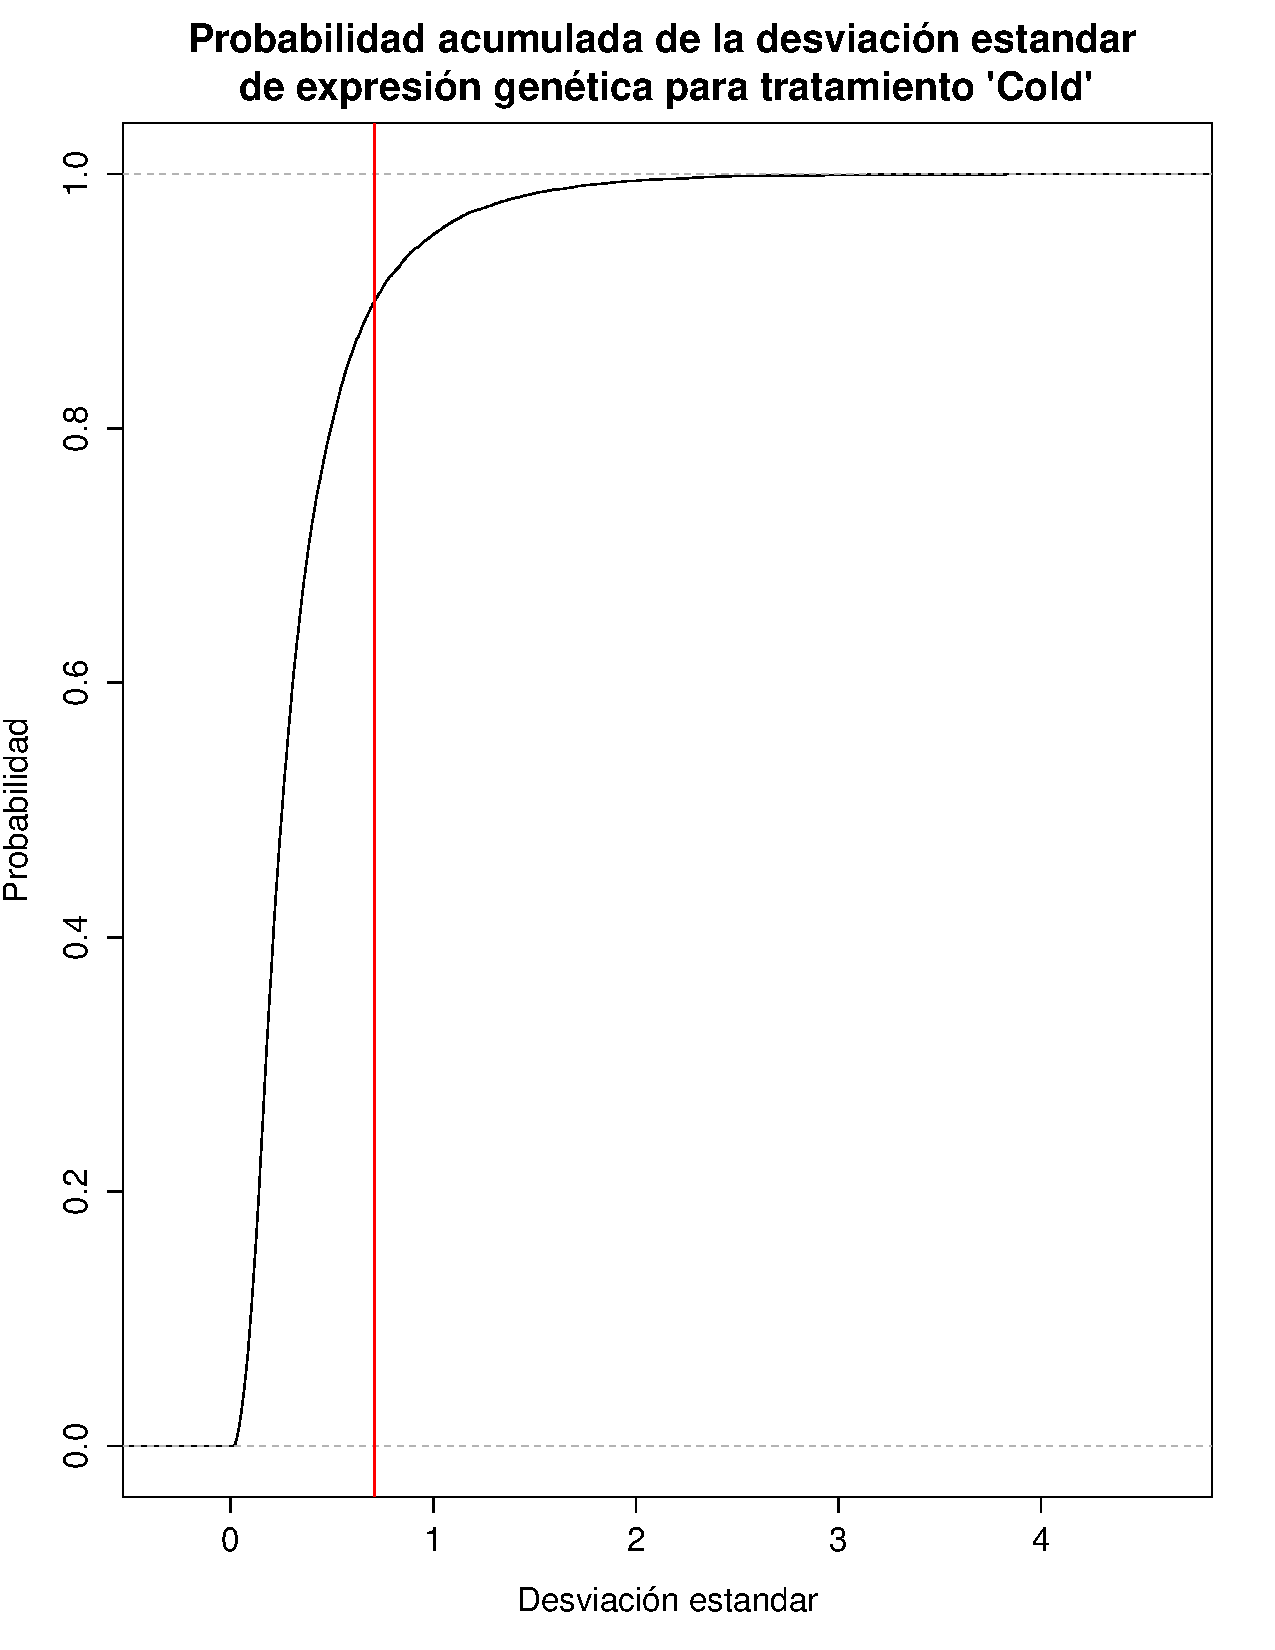
\includegraphics[width=1\textwidth]{densidad_de_desviacion_estandar}
    \caption{Distribución de probabilidad acumulada de la desviación estandar para los genes del tratamiento \textit{Cold}. Todos los genes con desviación estandar menor que la indicada por la recta vertical roja son descartados.}
    \label{fig:densidad_de_desviacion_estandar}
    \end{subfigure}
    \begin{subfigure}[t]{0.4\textwidth}
    \centering
    \includegraphics[width=1\textwidth]{densidad_para_niveles}
    \caption{distribución de probabilidad para los niveles de expresión para el tratamiento \textit{Cold}. La recta vertical roja muestra el valor a partir del cual se hace un corte.}
    \label{fig:densidad_para_niveles}
    \end{subfigure}
    \caption{Funciones de distribución de probabilidad para perfiles de expresión}
\end{figure*}
Una vez aplicados los fitros y obtenido los genes de mayor variabilidad en su expresión, se estandarizaron los datos obtenidos para poner a todos los genes en igualdad de condiciones y pesarlos de la misma forma en el agrupamiento. Un procedimiento normal de estandarización de genes para que cada gen tenga media cero y varianza unitaria implica realizar la transformación:
\begin{equation}
	\tilde{x_i} = \frac{x_i-\bar{x}}{\sigma_x}
\end{equation}
Con $x_i$ cada observación del gen $x$ a lo largo del tiempo para un determinado tratamiento. Una vez realizado el filtrado y estandarizado procedimos a agrupar los datos mediante los diferentes métodos mencionados en el capítulo 3.
\subsection{Agrupamiento con k-means}
\hl{ideas: poner aca que se probo con varios k para minimizar alguna funcion de costo. Mostrar de a pares las nubes de puntos y mostrar que k means solo puede ver por afuera de la nube de puntos, o quizas los perfiles que seguro sean los up y los down. y charlar un poco de la escala.}
\subsection{Agrupamiento con dynamic tree cut}
\hl{ideas: poner aca que se probo con deepsplit 1 y deepsplit 4. Que se logra meter mucho mejor, mostrar algunos perfiles para algun tratamiento para ambos y mostrar quizas una tabla con cada tratamiento cuantos clusters y que tamanios. charlar de nuevo sobre la escala.}
\subsection{Análisis de los métodos y problemas de escala de resolución}

\section{Coherencia entre la métrica transcripcional y otros espacios de conocimiento}
\hl{idea esperamos que los conocimientos (entendidos como nociones de similitud) de los distintos espacios sean diferentes pero no ortogonales...cuantificacion...veamos que estructuras son en cierto grado coherentes}
\subsection{Interacting densities}
\hl{genex1 /genex4  VS BPa/BPb/CC}
\hl{PINinfomap / KEGGinfomap/LCI para referencia}
\subsection{KTA y zKTA}
\hl{Global}
\hl{KTA Genex por tratamiento + PIN + KEGG + LCI / GOBPa, GOBPb, GOCC}
\hl{zKTA: por tratamiento Gx/GOBPa, Gx/GOBPb, Gx/GOCC, Gx/PIN, Gx/LCI, Gx/Kegg}